\documentclass[12pt]{report}
\usepackage{scribe,graphicx,graphics}
\usepackage{float}
\usepackage{siunitx}
\usepackage{braket}
\usepackage{mathabx}
\usepackage{listings}
\usepackage[bbgreekl]{mathbbol}
\course{CSE 389D} 	
\coursetitle{Mathematical Modeling}	
\semester{Spring 2025}
\lecturer{} % Due Date: {\bf Mon, Oct 3 2016}}
\lecturetitle{Problem Set}
\lecturenumber{4}   
\lecturedate{}    
\usepackage{enumerate}
\newcommand{\remind}[1]{\textcolor{red}{\textbf{#1}}} %To remind me of unfinished work to fix later
\newcommand{\hide}[1]{} %To hide large blocks of code without using % symbols

\newcommand{\ep}{\varepsilon}
\newcommand{\vp}{\varphi}
\newcommand{\lam}{\lambda}
\newcommand{\Lam}{\Lambda}
%\newcommand{\abs}[1]{\ensuremath{\left\lvert#1\right\rvert}} % This clashes with the physics package
%\newcommand{\norm}[1]{\ensuremath{\left\lVert#1\right\rVert}} % This clashes with the physics package
\newcommand{\floor}[1]{\ensuremath{\left\lfloor#1\right\rfloor}}
\newcommand{\ceil}[1]{\ensuremath{\left\lceil#1\right\rceil}}
\newcommand{\A}{\mathbb{A}}
\newcommand{\B}{\mathbb{B}}
\newcommand{\C}{\mathbb{C}}
\newcommand{\D}{\mathbb{D}}
\newcommand{\E}{\mathbb{E}}
\newcommand{\F}{\mathbb{F}}
\newcommand{\K}{\mathbb{K}}
\newcommand{\N}{\mathbb{N}}
\newcommand{\Q}{\mathbb{Q}}
\newcommand{\R}{\mathbb{R}}
\newcommand{\T}{\mathbb{T}}
\newcommand{\X}{\mathbb{X}}
\newcommand{\Y}{\mathbb{Y}}
\newcommand{\Z}{\mathbb{Z}}
\newcommand{\As}{\mathcal{A}}
\newcommand{\Bs}{\mathcal{B}}
\newcommand{\Cs}{\mathcal{C}}
\newcommand{\Ds}{\mathcal{D}}
\newcommand{\Es}{\mathcal{E}}
\newcommand{\Fs}{\mathcal{F}}
\newcommand{\Gs}{\mathcal{G}}
\newcommand{\Hs}{\mathcal{H}}
\newcommand{\Is}{\mathcal{I}}
\newcommand{\Js}{\mathcal{J}}
\newcommand{\Ks}{\mathcal{K}}
\newcommand{\Ls}{\mathcal{L}}
\newcommand{\Ms}{\mathcal{M}}
\newcommand{\Ns}{\mathcal{N}}
\newcommand{\Os}{\mathcal{O}}
\newcommand{\Ps}{\mathcal{P}}
\newcommand{\Qs}{\mathcal{Q}}
\newcommand{\Rs}{\mathcal{R}}
\newcommand{\Ss}{\mathcal{S}}
\newcommand{\Ts}{\mathcal{T}}
\newcommand{\Us}{\mathcal{U}}
\newcommand{\Vs}{\mathcal{V}}
\newcommand{\Ws}{\mathcal{W}}
\newcommand{\Xs}{\mathcal{X}}
\newcommand{\Ys}{\mathcal{Y}}
\newcommand{\Zs}{\mathcal{Z}}
\newcommand{\ab}{\textbf{a}}
\newcommand{\bb}{\textbf{b}}
\newcommand{\cb}{\textbf{c}}
\newcommand{\db}{\textbf{d}}
\newcommand{\ub}{\textbf{u}}
\newcommand{\sbb}{\textbf{s}}
%\renewcommand{\vb}{\textbf{v}} % This clashes with the physics package (the physics package already defines the \vb command)
\newcommand{\wb}{\textbf{w}}
\newcommand{\xb}{\textbf{x}}
\newcommand{\yb}{\textbf{y}}
\newcommand{\zb}{\textbf{z}}
\newcommand{\vbb}{\textbf{v}}
\newcommand{\Ab}{\textbf{A}}
\newcommand{\Bb}{\textbf{B}}
\newcommand{\Cb}{\textbf{C}}
\newcommand{\Db}{\textbf{D}}
\newcommand{\eb}{\textbf{e}}
\newcommand{\ex}{\textbf{e}_x}
\newcommand{\ey}{\textbf{e}_y}
\newcommand{\ez}{\textbf{e}_z}
\newcommand{\zerob}{\mathbf{0}}
\newcommand{\abar}{\overline{a}}
\newcommand{\bbar}{\overline{b}}
\newcommand{\cbar}{\overline{c}}
\newcommand{\dbar}{\overline{d}}
\newcommand{\ubar}{\overline{u}}
\newcommand{\vbar}{\overline{v}}
\newcommand{\wbar}{\overline{w}}
\newcommand{\xbar}{\overline{x}}
\newcommand{\ybar}{\overline{y}}
\newcommand{\zbar}{\overline{z}}
\newcommand{\Abar}{\overline{A}}
\newcommand{\Bbar}{\overline{B}}
\newcommand{\Cbar}{\overline{C}}
\newcommand{\Dbar}{\overline{D}}
\newcommand{\Ubar}{\overline{U}}
\newcommand{\Vbar}{\overline{V}}
\newcommand{\Wbar}{\overline{W}}
\newcommand{\Xbar}{\overline{X}}
\newcommand{\Ybar}{\overline{Y}}
\newcommand{\Zbar}{\overline{Z}}
\newcommand{\Aint}{A^\circ}
\newcommand{\Bint}{B^\circ}
\newcommand{\limk}{\lim_{k\to\infty}}
\newcommand{\limm}{\lim_{m\to\infty}}
\newcommand{\limn}{\lim_{n\to\infty}}
\newcommand{\limx}[1][a]{\lim_{x\to#1}}
\newcommand{\liminfm}{\liminf_{m\to\infty}}
\newcommand{\limsupm}{\limsup_{m\to\infty}}
\newcommand{\liminfn}{\liminf_{n\to\infty}}
\newcommand{\limsupn}{\limsup_{n\to\infty}}
\newcommand{\sumkn}{\sum_{k=1}^n}
\newcommand{\sumk}[1][1]{\sum_{k=#1}^\infty}
\newcommand{\summ}[1][1]{\sum_{m=#1}^\infty}
\newcommand{\sumn}[1][1]{\sum_{n=#1}^\infty}
\newcommand{\emp}{\varnothing}
\newcommand{\exc}{\backslash}
\newcommand{\sub}{\subseteq}
\newcommand{\sups}{\supseteq}
\newcommand{\capp}{\bigcap}
\newcommand{\cupp}{\bigcup}
\newcommand{\kupp}{\bigsqcup}
\newcommand{\cappkn}{\bigcap_{k=1}^n}
\newcommand{\cuppkn}{\bigcup_{k=1}^n}
\newcommand{\kuppkn}{\bigsqcup_{k=1}^n}
\newcommand{\cappk}[1][1]{\bigcap_{k=#1}^\infty}
\newcommand{\cuppk}[1][1]{\bigcup_{k=#1}^\infty}
\newcommand{\cappm}[1][1]{\bigcap_{m=#1}^\infty}
\newcommand{\cuppm}[1][1]{\bigcup_{m=#1}^\infty}
\newcommand{\cappn}[1][1]{\bigcap_{n=#1}^\infty}
\newcommand{\cuppn}[1][1]{\bigcup_{n=#1}^\infty}
\newcommand{\kuppk}[1][1]{\bigsqcup_{k=#1}^\infty}
\newcommand{\kuppm}[1][1]{\bigsqcup_{m=#1}^\infty}
\newcommand{\kuppn}[1][1]{\bigsqcup_{n=#1}^\infty}
\newcommand{\cappa}{\bigcap_{\alpha\in I}}
\newcommand{\cuppa}{\bigcup_{\alpha\in I}}
\newcommand{\kuppa}{\bigsqcup_{\alpha\in I}}
\newcommand{\Rx}{\overline{\mathbb{R}}}
\newcommand{\dx}{\,dx}
\newcommand{\dy}{\,dy}
\newcommand{\dt}{\,dt}
\newcommand{\dax}{\,d\alpha(x)}
\newcommand{\dbx}{\,d\beta(x)}
\DeclareMathOperator{\glb}{\text{glb}}
\DeclareMathOperator{\lub}{\text{lub}}
\newcommand{\xh}{\widehat{x}}
\newcommand{\yh}{\widehat{y}}
\newcommand{\zh}{\widehat{z}}
\newcommand{\<}{\langle}
\renewcommand{\>}{\rangle}
\renewcommand{\iff}{\Leftrightarrow}
\DeclareMathOperator{\im}{\text{im}}
\let\spn\relax\let\Re\relax\let\Im\relax
\DeclareMathOperator{\spn}{\text{span}}
\DeclareMathOperator{\sym}{\text{Sym}}
\DeclareMathOperator{\myskew}{\text{Skew}}
\DeclareMathOperator{\Re}{\text{Re}}
\DeclareMathOperator{\Im}{\text{Im}}
\DeclareMathOperator{\diag}{\text{diag}}
\endinput
\usepackage{xcolor}
\definecolor{codegreen}{rgb}{0,0.6,0}
\definecolor{codegray}{rgb}{0.5,0.5,0.5}
\definecolor{codepurple}{rgb}{0.58,0,0.82}
\definecolor{backcolour}{rgb}{0.95,0.95,0.92}

\lstdefinestyle{mystyle}{
    backgroundcolor=\color{backcolour},   
    commentstyle=\color{codegreen},
    keywordstyle=\color{magenta},
    numberstyle=\tiny\color{codegray},
    stringstyle=\color{codepurple},
    basicstyle=\ttfamily\footnotesize,
    breakatwhitespace=false,         
    breaklines=true,                 
    captionpos=b,                    
    keepspaces=true,                 
    numbers=left,                    
    numbersep=5pt,                  
    showspaces=false,                
    showstringspaces=false,
    showtabs=false,                  
    tabsize=2
}

\lstset{style=mystyle}
\usepackage{amsthm}
\newtheoremstyle{custom}
  {\topsep} % Space above
  {\topsep} % Space below
  {\upshape} % Body font
  {} % Indent amount
  {\itshape} % Theorem head font
  {.} % Punctuation after theorem head
  { } % Space after theorem head
  {} % Theorem head spec
\theoremstyle{custom}
\newtheorem{case}{Case}

% Insert your name here!
\scribe{Student Name: Noah Reef}
\newcommand{\rb}{\bold{r}}

\begin{document}
\maketitle


\section*{Problem 4.1}
\subsection*{Part a}
Recall that the spin operator is given by $\hat{S} = \frac{1}{2} \hbar \sigma$ where $\sigma = \bbsigma_x u_x + \bbsigma_y u_y + \bbsigma_z u_z$. Then we have that the expectation of the spin operator is
\begin{align*}
  \bra{\Psi}\hat{S} \ket{\Psi} = \frac{\hbar}{2}\left[\bra{\Psi}\bbsigma_x\ket{\Psi} u_x +\bra{\Psi}\bbsigma_y\ket{\Psi}u_y + \bra{\Psi}\bbsigma_z\ket{\Psi} u_z  \right]
\end{align*}
and we have that
\begin{align*}
  \bra{\Psi} \bbsigma_x \ket{\Psi} = \begin{bmatrix}u^*(r) &  d^*(r)\end{bmatrix} \begin{pmatrix}0 & 1 \\ 1 & 0 \end{pmatrix} \begin{bmatrix} u(r) \\ d(r) \end{bmatrix} &= u^*(r)d(r) + d^*(r)u(r) \\
                                                           &= \Re(u^*d) + i\Im(u^*d) + \Re(u^*d) - i\Im(u^*d) \\
                                                                      &= 2 \Re(u^*d)
\end{align*}
and
\begin{align*}
  \bra{\Psi} \bbsigma_y \ket{\Psi} = \begin{bmatrix}u^*(r) &  d^*(r)\end{bmatrix}\begin{pmatrix}0 & -i \\ i & 0 \end{pmatrix} \begin{bmatrix} u(r) \\ d(r) \end{bmatrix} &= -iu^*(r)d(r) + i d^*(r)u(r) \\ 
                                                           &= -i\Re(u^*d) + \Im(u^*d) + i \Re(u^*d) + \Im(u^*d) \\
                                                           &= 2 \Im(u^*d) 
\end{align*}
lastly,
\begin{align*}
  \bra{\Psi} \bbsigma_z \ket{\Psi} = \begin{bmatrix}u^*(r) &  d^*(r)\end{bmatrix}\begin{pmatrix}1 & 0 \\ 0 & -1 \end{pmatrix} \begin{bmatrix} u(r) \\ d(r) \end{bmatrix} &= u^*(r)u(r) - d^*(r)d(r) \\
                                                                     &= |u|^2 - |d|^2
\end{align*}
and hence then expectation value of the spin operator on this spinsor is given by
\begin{equation*}
  \bra{\Psi} \hat{S} \ket{\Psi} = \frac{\hbar}{2} \left[2\Re(u^*d) u_x + 2\Im(u^*d)u_y + (|u|^2 - |d|^2)u_z\right]
\end{equation*}

\subsection*{Part b}
We compute the norm of $\bra{\Psi}\hat{S}\ket{\Psi}$ as 
\begin{align*}
  |\bra{\Psi}\hat{S}\ket{\Psi}| &= \frac{\hbar}{2}\sqrt{4\Re(u^*d)^2 + 4 \Im(u^*d)^2 + |u|^4 - 2|u|^2|d|^2 + |d|^4} \\
                                &=\frac{\hbar}{2}\sqrt{4|u^*d|^2 + |u|^4 - 2|u|^2|d|^2 + |d|^4} \\
                                &=\frac{\hbar}{2}\sqrt{4|u|^2|d|^2 + |u|^4 - 2|u|^2|d|^2 + |d|^4}  \\
                                &=\frac{\hbar}{2}\sqrt{|u|^4 + 2|u|^2|d|^2 + |d|^4}  \\
                                &=\frac{\hbar}{2}\sqrt{(|u|^2 + |d|^2)^2} \\
                                &= \frac{\hbar}{2} \sqrt{|\Psi|^2} = \frac{\hbar}{2}   
\end{align*}

\subsection*{Part c}
Consider
\begin{equation*}
  \exp\left(i \varphi \frac{\hat{S}_z}{\hbar}\right) = \sum_{n=0}^\infty \frac{\left (i \varphi \frac{\hat{S}_z}{\hbar}\right)^n}{n!} = \sum_{n=0}^\infty \frac{1}{n!}\left(\frac{i\varphi}{2}\right)^n \begin{pmatrix}1 & 0 \\ 0 & -1 \end{pmatrix}^n
\end{equation*}
note that for $n$ even we have that
\begin{equation*}
  \begin{pmatrix} 1 & 0 \\ 0 & -1\end{pmatrix}^n = \begin{pmatrix}1 & 0 \\ 0 & 1 \end{pmatrix}
\end{equation*}
and remains unchanged for $n$ odd, thus we can write the above as
\begin{equation*}
  \exp\left(i \varphi \frac{\hat{S}_z}{\hbar}\right) = \begin{pmatrix}\sum_{n=0}^\infty \frac{1}{n!}\left(\frac{i\varphi}{2}\right)^n & 0 \\
    0 & \sum_{n=0}^\infty \frac{1}{n!}\left(-\frac{i\varphi}{2}\right)^n \end{pmatrix} = \begin{pmatrix} \exp\left(\frac{i\varphi}{2}\right) & 0 \\ 0 & \exp\left(-\frac{i\varphi}{2}\right)\end{pmatrix}
\end{equation*}

\subsection*{Part d}
Note that
\begin{equation*}
\Psi' =\exp\left(i \varphi \frac{\hat{S}_z}{\hbar}\right) \Psi =  \begin{pmatrix} \exp\left(\frac{i\varphi}{2}\right) & 0 \\ 0 & \exp\left(-\frac{i\varphi}{2}\right)\end{pmatrix} \begin{bmatrix} u \\ d\end{bmatrix} = \begin{bmatrix} e^{i\varphi/2} u \\ e^{-i\varphi/2}d \end{bmatrix} 
\end{equation*}
then we get that
\begin{align*}
  \bra{\Psi} \bbsigma_x \ket{\Psi} &= \begin{bmatrix}e^{-i\varphi/2}u^*(r) &  e^{i\varphi/2}d^*(r)\end{bmatrix} \begin{pmatrix}0 & 1 \\ 1 & 0 \end{pmatrix} \begin{bmatrix} e^{i\varphi/2}u(r) \\ e^{-i\varphi/2}d(r) \end{bmatrix} = e^{-i\varphi}u^*(r)d(r) + e^{i\varphi}d^*(r)u(r) \\
                                                                          &= \Re(e^{-i\varphi}u^*d) + i\Im(e^{-i\varphi}u^*d) + \Re(e^{-i\varphi}u^*d) - i\Im(e^{-i\varphi}u^*d) \\
                                                                      &= 2 \Re(e^{-i\varphi}u^*d)
\end{align*}
and
\begin{align*}
  \bra{\Psi} \bbsigma_y \ket{\Psi} &= \begin{bmatrix}e^{-i\varphi/2}u^*(r) &  e^{i\varphi/2}d^*(r)\end{bmatrix}\begin{pmatrix}0 & -i \\ i & 0 \end{pmatrix} \begin{bmatrix} e^{i\varphi/2}u(r) \\ e^{-i\varphi/2}d(r) \end{bmatrix} = -ie^{i\varphi}u^*(r)d(r) + i e^{i\varphi}d^*(r)u(r) \\ 
                                   &= -i\Re(e^{-i\varphi}u^*d) + \Im(e^{-i\varphi}u^*d) + i \Re(e^{-i\varphi}u^*d) + \Im(e^{-i\varphi}u^*d) \\
                                                           &= 2 \Im(e^{-i\varphi}u^*d) 
\end{align*}
lastly,
\begin{align*}
  \bra{\Psi} \bbsigma_z \ket{\Psi} = \begin{bmatrix}e^{-i\varphi/2}u^*(r) &  e^{i\varphi/2}d^*(r)\end{bmatrix}\begin{pmatrix}1 & 0 \\ 0 & -1 \end{pmatrix} \begin{bmatrix} e^{i\varphi/2}u(r) \\ e^{-i\varphi/2}d(r) \end{bmatrix} &= u^*(r)u(r) - d^*(r)d(r) \\
                                                                     &= |u|^2 - |d|^2
\end{align*}
and hence then expectation value of the spin operator on this spinsor is given by
\begin{equation*}
  \bra{\Psi'} \hat{S} \ket{\Psi'} = \frac{\hbar}{2} \left[2\Re(e^{-i\varphi}u^*d) u_x + 2\Im(e^{-i\varphi}u^*d)u_y + (|u|^2 - |d|^2)u_z\right]
\end{equation*}

\subsection*{Part e}
Suppose that $u^*d = a + bi$ then $a = \frac{1}{2}S_x$ and $b = \frac{1}{2}S_y$ and we have that 
\begin{equation*}
  e^{-i\varphi} u^*d = (a + bi)(\cos(i\varphi) - i\sin(\varphi)) = a\cos(\varphi) + b\sin(\varphi) + i \left(b\cos(\varphi) - a\sin(\varphi)\right)
\end{equation*}
thus
\begin{equation*}
  S'_x = 2\Re(e^{-i\varphi}u^*d) = S_x \cos(\varphi) + S_y \sin(\varphi)
\end{equation*}
and
\begin{equation*}
  S'_y = 2\Im(e^{-i\varphi}u^*d) = S_y\cos(\varphi) - S_x\sin(\varphi)
\end{equation*}
and clearly
\begin{equation*}
  S'_z = S_z
\end{equation*}

\subsection*{Part f}
From the change of coordinates in Part e, we have that $ \exp\left(i \varphi \frac{\hat{S}_z}{\hbar}\right)$ is a clockwise rotation about the $z$-axis by angle $\varphi$.  

\section*{Problem 4.2}
\subsection*{Part a}
Recall that 
\begin{equation*}
  \chi_\uparrow = \begin{bmatrix}
    1 \\ 0
  \end{bmatrix} \quad \text{and} \quad \chi_\downarrow = \begin{bmatrix}
    0 \\ 1
    \end{bmatrix}
\end{equation*}
and note that 
\begin{align*}
\chi_{\uparrow} \otimes \chi_{\uparrow} &= \begin{bmatrix}
    1 \\ 0
  \end{bmatrix} \otimes \begin{bmatrix}
    1 \\ 0
  \end{bmatrix} = \begin{bmatrix}
    1 \\ 0 \\ 0 \\ 0
  \end{bmatrix} \\
\chi_{\uparrow} \otimes \chi_{\downarrow} &= \begin{bmatrix}
    1 \\ 0
  \end{bmatrix} \otimes \begin{bmatrix}
    0 \\ 1
  \end{bmatrix} = \begin{bmatrix}
    0 \\ 1 \\ 0 \\ 0
  \end{bmatrix} \\
\chi_{\downarrow} \otimes \chi_{\uparrow} &= \begin{bmatrix}
    0 \\ 1
  \end{bmatrix} \otimes \begin{bmatrix}
    1 \\ 0
  \end{bmatrix} = \begin{bmatrix}
    0 \\ 0 \\ 1 \\ 0
  \end{bmatrix} \\
  \chi_{\downarrow} \otimes \chi_{\downarrow} &= \begin{bmatrix}
    0 \\ 1
  \end{bmatrix} \otimes \begin{bmatrix}
    0 \\ 1
  \end{bmatrix} = \begin{bmatrix}
    0 \\ 0 \\ 0 \\ 1
  \end{bmatrix}
\end{align*}
and hence we see that
\begin{align*}
  \psi(\rb_1,\rb_2; 1) \chi_{\uparrow} \otimes \chi_{\uparrow} + \psi(\rb_1,\rb_2; 2) \chi_{\uparrow} \otimes \chi_{\downarrow} + \psi(\rb_1,\rb_2; 3) \chi_{\downarrow} \otimes \chi_{\uparrow} + \psi(\rb_1,\rb_2; 4) \chi_{\downarrow} \otimes \chi_{\downarrow} 
\end{align*}
becomes
\begin{equation*}
    \psi(\rb_1,\rb_2; 1)\begin{bmatrix}
    1 \\ 0 \\ 0 \\ 0
  \end{bmatrix}  + \psi(\rb_1,\rb_2; 2) \begin{bmatrix}
  0 \\ 1 \\ 0 \\ 0
\end{bmatrix}  + \psi(\rb_1,\rb_2; 3) \begin{bmatrix}
0 \\ 0 \\ 1 \\ 0
\end{bmatrix} + \psi(\rb_1,\rb_2; 4) \begin{bmatrix}
0 \\ 0 \\ 0 \\ 1\end{bmatrix}  = \begin{bmatrix}
  \psi(\rb_1,\rb_2; 1) \\
  \psi(\rb_1,\rb_2; 2) \\
  \psi(\rb_1,\rb_2; 3) \\
  \psi(\rb_1,\rb_2; 4)
\end{bmatrix}
\end{equation*}

\subsection*{Part b}
To compute $(\hat{S}_{\text{tot}}))_z$ we compute 
\begin{equation*}
(\hat{S}_{\text{tot}})_z = S_z \otimes I + I \otimes S_z = \frac{\hbar}{2} \left(\bbsigma_z \otimes I + I \otimes \bbsigma_z\right)
\end{equation*}
then we have that
\begin{align*}
\bbsigma_z \otimes I &= \begin{pmatrix} 1 & 0 \\ 0 & -1 \end{pmatrix} \otimes \begin{pmatrix} 1 & 0 \\ 0 & 1 \end{pmatrix} = \begin{pmatrix} 1 & 0 & 0 & 0 \\ 0 & 1 & 0 & 0 \\ 0 & 0 & -1 & 0 \\ 0 & 0 & 0 & -1 \end{pmatrix} \\
I \otimes \bbsigma_z &= \begin{pmatrix} 1 & 0 \\ 0 & 1 \end{pmatrix} \otimes \begin{pmatrix} 1 & 0 \\ 0 & -1 \end{pmatrix} = \begin{pmatrix} 1 & 0 & 0 & 0 \\ 0 & -1 & 0 & 0 \\ 0 & 0 & 1 & 0 \\ 0 & 0 & 0 & -1 \end{pmatrix}
\end{align*}
then we have that
\begin{equation*}
  (\hat{S}_{\text{tot}})_z = \frac{\hbar}{2} \begin{pmatrix} 2 & 0 & 0 & 0 \\ 0 & 0 & 0 & 0 \\ 0 & 0 & 0 & 0 \\ 0 & 0 & 0 & -2 \end{pmatrix} = \hbar \begin{pmatrix} 1 & 0 & 0 & 0 \\ 0 & 0 & 0 & 0 \\ 0 & 0 & 0 & 0 \\ 0 & 0 & 0 & -1 \end{pmatrix}
\end{equation*}
Note that doing a similar process for $(S_{\text{tot}})_x$ and $(S_{\text{tot}})_y$ we get that
\begin{align*}
  (\hat{S}_{\text{tot}})_x &= \frac{\hbar}{2} \begin{pmatrix}0 & 1 & 1 & 0 \\ 1 & 0 & 0 & 1 \\ 1 & 0 & 0 & 1 \\ 0 & 1 & 1 & 0 \end{pmatrix} \\
(\hat{S}_{\text{tot}})_y &= \frac{\hbar}{2} \begin{pmatrix} 0 & -i & -i & 0 \\ i & 0 & 0 & -i \\ i & 0 & 0 & -i \\ 0 & i & i & 0\end{pmatrix}
\end{align*}
so then we have that
\begin{equation*}
S_{\text{tot}}^2 = (\hat{S}_{\text{tot}})_x^2 + (\hat{S}_{\text{tot}})_y^2 + (\hat{S}_{\text{tot}})_z^2 = \begin{pmatrix}2\hbar^2 & 0 & 0 & 0 \\ 0 & \hbar^2 & \hbar^2 & 0 \\ 0 & \hbar^2 & \hbar^2 & 0 \\ 0 & 0 & 0 & 2\hbar^2\end{pmatrix} 
\end{equation*}
\subsection*{Part c} 
Consider

\begin{align*}
  \Psi_1 &= f(\rb_1,\rb_2) \chi_{\uparrow} \otimes \chi_{\uparrow} \\
  \Psi_2 &= f(\rb_1,\rb_2) \chi_{\uparrow} \otimes \chi_{\downarrow} \\
  \Psi_3 &= f(\rb_1,\rb_2) \chi_{\downarrow} \otimes \chi_{\uparrow} \\
  \Psi_4 &= f(\rb_1,\rb_2) \chi_{\downarrow} \otimes \chi_{\downarrow} 
\end{align*}

Then we have that 
\begin{align*}
\bra{\Psi_1}S_{\text{tot}}^2 \ket{\Psi_1} &= \int \begin{bmatrix} f^*(\rb_1,\rb_2) & 0 & 0 & 0 \end{bmatrix} \begin{pmatrix}2\hbar^2 & 0 & 0 & 0 \\ 0 & \hbar^2 & \hbar^2 & 0 \\ 0 & \hbar^2 & \hbar^2 & 0 \\ 0 & 0 & 0 & 2\hbar^2\end{pmatrix}  \begin{bmatrix} f(\rb_1,\rb_2) \\ 0 \\ 0 \\ 0 \end{bmatrix} d\rb_1 d\rb_2 \\
                                          &=  \int 2\hbar^2 |f(\rb_1,\rb_2)|^2 d\rb_1 d\rb_2  = 2\hbar^2 
\end{align*}
\begin{align*}
\bra{\Psi_2}S_{\text{tot}}^2 \ket{\Psi_2} &= \int \begin{bmatrix} 0 & f^*(\rb_1,\rb_2) & 0 & 0 \end{bmatrix} \begin{pmatrix}2\hbar^2 & 0 & 0 & 0 \\ 0 & \hbar^2 & \hbar^2 & 0 \\ 0 & \hbar^2 & \hbar^2 & 0 \\ 0 & 0 & 0 & 2\hbar^2\end{pmatrix}  \begin{bmatrix} 0 \\ f(\rb_1,\rb_2)\\ 0 \\ 0 \end{bmatrix} d\rb_1 d\rb_2 \\
                                          &=  \int \hbar^2 |f(\rb_1,\rb_2)|^2 d\rb_1 d\rb_2 = \hbar^2
\end{align*}
\begin{align*}
  \bra{\Psi_3}S_{\text{tot}}^2 \ket{\Psi_3} &= \int \begin{bmatrix} 0 & 0 & f^*(\rb_1,\rb_2) & 0 \end{bmatrix} \begin{pmatrix}2\hbar^2 & 0 & 0 & 0 \\ 0 & \hbar^2 & \hbar^2 & 0 \\ 0 & \hbar^2 & \hbar^2 & 0 \\ 0 & 0 & 0 & 2\hbar^2\end{pmatrix}  \begin{bmatrix} 0 \\ 0 \\ f(\rb_1,\rb_2)\\ 0 \end{bmatrix} d\rb_1 d\rb_2 \\
                                            &=  \int \hbar^2 |f(\rb_1,\rb_2)|^2 d\rb_1 d\rb_2 = \hbar^2
\end{align*}
\begin{align*}
  \bra{\Psi_4}S_{\text{tot}}^2 \ket{\Psi_4} &= \int \begin{bmatrix} 0 & 0 & 0 & f^*(\rb_1,\rb_2) \end{bmatrix} \begin{pmatrix}2\hbar^2 & 0 & 0 & 0 \\ 0 & \hbar^2 & \hbar^2 & 0 \\ 0 & \hbar^2 & \hbar^2 & 0 \\ 0 & 0 & 0 & 2\hbar^2\end{pmatrix}  \begin{bmatrix} 0 \\ 0 \\ 0 \\ f(\rb_1,\rb_2) \end{bmatrix} d\rb_1 d\rb_2 \\
                                            &=  \int 2\hbar^2 |f(\rb_1,\rb_2)|^2 d\rb_1 d\rb_2 = 2\hbar^2
\end{align*}

\subsection*{Part d}
\begin{align*}
  \bra{\Psi_1}(S_{\text{tot}})_z \ket{\Psi_1} &= \int \begin{bmatrix} f^*(\rb_1,\rb_2) & 0 & 0 & 0 \end{bmatrix} \begin{pmatrix} \hbar & 0 & 0 & 0 \\ 0 & 0 & 0 & 0 \\ 0 & 0 & 0 & 0 \\ 0 & 0 & 0 & -\hbar \end{pmatrix}\begin{bmatrix} f(\rb_1,\rb_2) \\ 0 \\ 0 \\ 0 \end{bmatrix} d\rb_1 d\rb_2 \\
                                            &=  \int \hbar |f(\rb_1,\rb_2)|^2 d\rb_1 d\rb_2  = \hbar 
  \end{align*}
  \begin{align*}
  \bra{\Psi_2}(S_{\text{tot}})_z \ket{\Psi_2} &= \int \begin{bmatrix} 0 & f^*(\rb_1,\rb_2) & 0 & 0 \end{bmatrix}  \begin{pmatrix} \hbar & 0 & 0 & 0 \\ 0 & 0 & 0 & 0 \\ 0 & 0 & 0 & 0 \\ 0 & 0 & 0 & -\hbar \end{pmatrix} \begin{bmatrix} 0 \\ f(\rb_1,\rb_2)\\ 0 \\ 0 \end{bmatrix} d\rb_1 d\rb_2 \\
                                            &=  0
  \end{align*}
  \begin{align*}
    \bra{\Psi_3}(S_{\text{tot}})_z \ket{\Psi_3} &= \int \begin{bmatrix} 0 & 0 & f^*(\rb_1,\rb_2) & 0 \end{bmatrix}  \begin{pmatrix} \hbar & 0 & 0 & 0 \\ 0 & 0 & 0 & 0 \\ 0 & 0 & 0 & 0 \\ 0 & 0 & 0 & -\hbar \end{pmatrix}\begin{bmatrix} 0 \\ 0 \\ f(\rb_1,\rb_2)\\ 0 \end{bmatrix} d\rb_1 d\rb_2 \\
                                              &=  0
  \end{align*}
  \begin{align*}
    \bra{\Psi_4}(S_{\text{tot}})_z \ket{\Psi_4} &= \int \begin{bmatrix} 0 & 0 & 0 & f^*(\rb_1,\rb_2) \end{bmatrix}  \begin{pmatrix} \hbar & 0 & 0 & 0 \\ 0 & 0 & 0 & 0 \\ 0 & 0 & 0 & 0 \\ 0 & 0 & 0 & -\hbar \end{pmatrix}  \begin{bmatrix} 0 \\ 0 \\ 0 \\ f(\rb_1,\rb_2) \end{bmatrix} d\rb_1 d\rb_2 \\
                                              &=  -\int \hbar |f(\rb_1,\rb_2)|^2 d\rb_1 d\rb_2 = -\hbar
  \end{align*}

\subsection*{Part e}
For $\Psi(\rb_1,\rb_2) = f(\rb_1,\rb_2) \chi_1 \otimes \chi_2$ to be antisymmetric, we require that $\Psi(\rb_1,\rb_2) = - \Psi(\rb_2,\rb_1)$. This means that we require
\begin{equation*}
f(\rb_1,\rb_2) \chi_1 \otimes \chi_2 = -f(\rb_2,\rb_1) \chi_2 \otimes \chi_1
\end{equation*}
that is if $\chi_1 \otimes \chi_2 = \chi_2 \otimes \chi_1$ (i.e. $\chi_1 = \chi_2$) then we have that we require $f(\rb_1, \rb_2) = -f(\rb_2,\rb_1)$, that is $f$ must be antisymmetric.  

\subsection*{Part f}

We wish to show that the two–electron spinors
\[
\Psi_a(\mathbf{r}_1,\mathbf{r}_2) = f_a(\mathbf{r}_1,\mathbf{r}_2) \Bigl(\chi_\uparrow\otimes\chi_\downarrow + \chi_\downarrow\otimes\chi_\uparrow\Bigr),
\]
\[
\Psi_s(\mathbf{r}_1,\mathbf{r}_2) = f_s(\mathbf{r}_1,\mathbf{r}_2) \Bigl(\chi_\uparrow\otimes\chi_\downarrow - \chi_\downarrow\otimes\chi_\uparrow\Bigr),
\]
fulfill Pauli's principle, swapping $\rb_1$ with $\rb_2$ yields
\[
\Psi_a(\mathbf{r}_2,\mathbf{r}_1) = f_a(\mathbf{r}_2,\mathbf{r}_1)Bigl(\chi_\uparrow\otimes\chi_\downarrow + \chi_\downarrow\otimes\chi_\uparrow\Bigr) = -f(\rb_1,\rb_2)\Bigl(\chi_\uparrow\otimes\chi_\downarrow + \chi_\downarrow\otimes\chi_\uparrow\Bigr).
\]
Thus, \(\Psi_a\) is antisymmetric under electron exchange.
Similarly, under exchange we have
\[
\Psi_s(\mathbf{r}_2,\mathbf{r}_1) = f_s(\mathbf{r}_2,\mathbf{r}_1) \Bigl(\chi_\uparrow\otimes\chi_\downarrow - \chi_\downarrow\otimes\chi_\uparrow\Bigr).
\]
Since \( f_s \) is symmetric, and recalling that the spin singlet is antisymmetric, we obtain
\[
\Psi_s(\mathbf{r}_2,\mathbf{r}_1) = f_s(\mathbf{r}_1,\mathbf{r}_2) \Bigl[-\bigl(\chi_\uparrow\otimes\chi_\downarrow - \chi_\downarrow\otimes\chi_\uparrow\bigr)\Bigr]
= - f_s(\mathbf{r}_1,\mathbf{r}_2) \Bigl(\chi_\uparrow\otimes\chi_\downarrow - \chi_\downarrow\otimes\chi_\uparrow\bigr)
= - \Psi_s(\mathbf{r}_1,\mathbf{r}_2).
\]
Thus, \(\Psi_s\) is also antisymmetric. Thus the wavefunction satisfy
\[
\Psi(\mathbf{r}_2,\mathbf{r}_1) = -\Psi(\mathbf{r}_1,\mathbf{r}_2),
\]



\subsection*{Part g}
\begin{align*}
    \Psi_1 &= f(\rb_1,\rb_2) \chi_{\uparrow} \otimes \chi_{\uparrow} \\
    \Psi_2 &= f(\rb_1,\rb_2) \frac{1}{\sqrt{2}}(\chi_{\uparrow} \otimes \chi_{\downarrow} + \chi_{\downarrow} \otimes \chi_{\uparrow}) \\
    \Psi_3 &= f(\rb_1,\rb_2) \chi_{\downarrow} \otimes \chi_{\downarrow} \\
    \Psi_4 &= f(\rb_1,\rb_2) (\chi_{\uparrow} \otimes \chi_{\downarrow} - \chi_{\downarrow} \otimes \chi_{\uparrow}) \\
\end{align*}
then we see that
\begin{align*}
    \bra{\Psi_1}(S_{tot})_z\ket{\Psi_1} &= \hbar \\
    \bra{\Psi_1}S_{tot}^2\ket{\Psi_1} &= 2\hbar^2
\end{align*}
and
\begin{align*}
    \bra{\Psi_2}(S_{tot})_z\ket{\Psi_2} &= 0 + 0 = 0 \\
    \bra{\Psi_2}S_{tot}^2\ket{\Psi_2} &= \frac{2\hbar^2}{2} + \frac{2\hbar^2}{2} = 2\hbar^2
\end{align*}
and
\begin{align*}
    \bra{\Psi_3}(S_{tot})_z\ket{\Psi_3} &= -\hbar \\
    \bra{\Psi_3}S_{tot}^2\ket{\Psi_3} &= \frac{2\hbar^2}{2} + \frac{2\hbar^2}{2} = 2\hbar^2
\end{align*}
and lastly,
\begin{align*}
    \bra{\Psi_4}(S_{tot})_z\ket{\Psi_4} &= 0 - 0 = 0 \\
    \bra{\Psi_4}S_{tot}^2\ket{\Psi_4} &= \frac{2\hbar^2}{2} - \frac{2\hbar^2}{2} = 0
\end{align*}
\section*{Problem 4.3}
\subsection*{Part a}
Consider the singlet spinor Slater determinant given by
\begin{equation*}
    \psi(1,2) = \phi(1)\phi(2) \frac{1}{\sqrt{2}} \left(\chi_{\uparrow} \otimes \chi_{\downarrow} - \chi_{\downarrow} \otimes \chi_{\uparrow}\right)
\end{equation*}
recall that
\begin{equation*}
\chi_{\uparrow} \otimes \chi_{\downarrow}  = \begin{bmatrix}
    0 \\ 1 \\ 0 \\ 0
  \end{bmatrix} \quad \text{and} \quad 
\chi_{\downarrow} \otimes \chi_{\uparrow} = \begin{bmatrix}
    0 \\ 0 \\ 1 \\ 0
  \end{bmatrix} 
\end{equation*}
thus
\begin{equation*}
 \psi(1,2) = \phi(1)\phi(2) \frac{1}{\sqrt{2}} \left(\begin{bmatrix}
    0 \\ 1 \\ 0 \\ 0
  \end{bmatrix} -  \begin{bmatrix}
    0 \\ 0 \\ 1 \\ 0
  \end{bmatrix} \right) = \phi(1)\phi(2) \frac{1}{\sqrt{2}} \begin{bmatrix}
    \phantom{-}0 \\ \phantom{-}1 \\ -1 \\ \phantom{-}0
  \end{bmatrix}
\end{equation*}
similarly we find that
\begin{equation*}
\psi(2,1) = \phi(1)\phi(2) \frac{1}{\sqrt{2}}\left(\chi_{\downarrow} \otimes \chi_{\uparrow} - \chi_{\uparrow} \otimes \chi_{\downarrow}\right) = \phi(1)\phi(2) \frac{1}{\sqrt{2}} \begin{bmatrix}
    \phantom{-}0 \\ -1 \\ \phantom{-}1 \\ \phantom{-}0
  \end{bmatrix} = -\psi(1,2)
\end{equation*}
hence $\psi$ is anti-symmetric.

\subsection*{Part b}
For $\psi$ to be normalized we require that,
\begin{align*}
\braket{\psi|\psi} = \int \,d1 d2 \psi^*\psi = \int \, d1 d2 |\phi(1)|^2 |\phi(2)|^2 = \left(\int \, dr |\phi(r)|^2\right)^2 = 1
\end{align*}
which implies that
\begin{equation*}
\int \, dr |\phi(r)|^2 = 1
\end{equation*}
hence for $\psi$ to be normalized, $\phi$ must also be normalized.

\subsection*{Part c}
Suppose we have the following Hamiltonian,
\begin{equation*}
\hat{H} = \hat{H}_0(r) + \hat{H}_0(r') + \frac{\beta}{|r - r'|}
\end{equation*}
where
\begin{equation*}
    \hat{H}_0(r) = -\frac{\hbar^2 \nabla^2}{2m} - \frac{2\beta}{|r|} \quad \text{and} \quad \beta = \frac{e^2}{4\pi \epsilon_0} 
\end{equation*}
then we see that 
\begin{equation*}
    \bra{\psi}\hat{H}\ket{\psi} = \bra{\psi}\hat{H}_0(r) \ket{\psi} + \bra{\psi}\hat{H}_0(r') \ket{\psi} + \beta \bra{\psi} \frac{1}{r-r'} \ket{\psi}
\end{equation*}
additionally we see that
\begin{align*}
    \bra{\psi} \hat{H}_0(r) \ket{\psi} &= \frac{1}{2}\int \, dr dr'\begin{bmatrix}
    \phantom{-}0 & \phantom{-}1 & -1 & \phantom{-}0
  \end{bmatrix}\begin{bmatrix}
    \phantom{-}0 \\ \phantom{-}1 \\ -1 \\ \phantom{-}0
  \end{bmatrix} |\phi(r')|^2 \phi^*(r) \hat{H}_0(r) \phi(r) \\
  &= \int \, dr dr' |\phi(r')|^2 \phi^*(r) \hat{H}_0(r) \phi(r) = \int \, dr' |\phi(r')|^2 \int \, dr \phi^*(r) \hat{H}_0(r) \phi(r)\\
  &= \int \, dr \phi^*(r) \hat{H}_0(r) \phi(r)
\end{align*}
we can do a similar process for $\bra{\psi} \hat{H}_0(r') \ket{\psi}$ and we get that
\begin{equation*}
\bra{\psi} \hat{H}_0(r) \ket{\psi} + \bra{\psi} \hat{H}_0(r') \ket{\psi} = 2\int \, dr \phi^*(r) \hat{H}_0(r) \phi(r)
\end{equation*}
lastly for the last term we get that
\begin{align*}
    \beta \bra{\psi} \frac{1}{r-r'} \ket{\psi} &= \frac{\beta}{2} \int \, dr dr' \frac{\phi^*(r)\phi(r)\phi^*(r')\phi(r')}{|r - r'|} \begin{bmatrix}
    \phantom{-}0 & \phantom{-}1 & -1 & \phantom{-}0
  \end{bmatrix}\begin{bmatrix}
    \phantom{-}0 \\ \phantom{-}1 \\ -1 \\ \phantom{-}0
  \end{bmatrix} \\
  &= \beta \int\int \, dr dr' \frac{\phi^*(r)\phi(r)\phi^*(r')\phi(r')}{|r - r'|}
\end{align*}
hence we have that 
\begin{equation*}
    E = \bra{\psi} \hat{H} \ket{\psi} =  2\int \, dr \phi^*(r) \hat{H}_0(r) \phi(r) + \beta \int\int \, dr dr' \frac{\phi^*(r)\phi(r)\phi^*(r')\phi(r')}{|r - r'|}
\end{equation*}
\subsection*{Part d}
Recall that we can write the minimization of $E$ with respect to $\phi^*(r)$ subject to the normalization constraint via the Lagrangian as,
\begin{equation*}
L = E - \lambda \left(\int \, dr |\phi(r)|^2 - 1\right)
\end{equation*}
and we wish to find $\phi(r)$ such that 
\begin{equation*}
\frac{\delta L}{\delta \phi^*(r)} = \frac{\delta E}{\delta \phi^*(r)} - \frac{\delta}{\delta \phi^*(r)} \lambda \left(\int \, dr \phi^*(r)\phi(r) - 1\right) = 0
\end{equation*}
Note that for the first term, we have that 
\begin{align*}
&\frac{d}{d\epsilon}|_{\epsilon = 0} \left(2\int \, dr [\phi(r) + \epsilon \delta(r' - r)]^* \hat{H}_0(r) \phi(r) \right) =   2 \hat{H}_0(r) \phi(r)\\
&\frac{d}{d\epsilon}|_{\epsilon = 0} \left(\beta \int \, dr dr' \frac{[\phi(r) + \epsilon \delta(r - r')]^*\phi(r)[\phi(r') + \epsilon \delta(r' - r)]^*\phi(r')}{|r - r'|}\right) \\ &=
 \beta \int \int \, drdr' \frac{\delta(r -r')\phi(r)\phi^*(r')\phi(r')}{|r-r'|} + \beta \int \int \, drdr' \frac{\phi^*(r)\phi(r)\delta(r'-r)\phi(r')}{|r-r'|} \\ 
 &= \beta \int \int \, drdr' \frac{\delta(r-r')\phi(r)\phi^*(r')\phi(r')}{|r-r'|} + \beta \int \int \, drdr' \frac{\phi^*(r)\phi(r)\delta(r'-r)\phi(r')}{|r-r'|} \\ 
 &= 2\beta \phi(r) \int \, dr' \frac{|\phi(r')|^2}{|r-r'|}
\end{align*}
lastly we get that
\begin{equation*}
\frac{\delta}{\delta \phi^*(r)} \lambda \left(\int \, dr \phi^*(r)\phi(r) - 1\right) = \lambda \frac{d}{d\epsilon}|_{\epsilon = 0} \int \, dr [\phi(r) + \epsilon\delta(r-r')]^*\phi(r) = \lambda \phi(r)
\end{equation*}
so then by re-arranging terms we get that
\begin{equation*}
      \hat{H}_0(r) \phi(r) + \beta \phi(r) \int \, dr' \frac{|\phi(r')|^2}{|r-r'|} = \frac{\lambda}{2} \phi(r) = \epsilon \phi(r)
\end{equation*}
or
\begin{equation*}
    -\frac{\hbar^2}{2m}\nabla^2\phi(r) + \left[-\frac{2e^2}{4\pi \epsilon_0 |r|} + \int \, dr' \frac{e^2 |\phi(r')|^2}{4\pi \epsilon_0 |r-r'|}\right] \phi(r) = \epsilon \phi(r)
\end{equation*}

\subsection*{Part e}
Consider the effective potential,
\begin{equation*}
    V_{\text{eff}}(r) = -\frac{2e^2}{4\pi \epsilon_0 |r|} + \int \, dr' \frac{e^2 |\phi(r')|^2}{4\pi \epsilon_0 |r-r'|}
\end{equation*}
Now if we consider the case where $|r| \to 0$, we see that 
\begin{equation*}
    \frac{2e^2}{4\pi \epsilon_0 |r|} \to \infty \quad \text{and} \quad \int \, dr' \frac{e^2 |\phi(r')|^2}{4\pi \epsilon_0 |r-r'|} \to \int \, dr' \frac{e^2 |\phi(r')|^2}{4\pi \epsilon_0 |r'|} < \infty
\end{equation*}
hence for sufficiently small $r$ we have that the right-hand term dominates and hence the potential behaves as
\begin{equation*}
V_{\text{eff}}(r) \sim -\frac{Ze^2}{4\pi \epsilon_0 |r|}  
\end{equation*}
where $Z = 2$. Now if $|r| \to \infty$ we have that for sufficiently large $r$, $|r-r'| \sim |r|$ and hence
\begin{equation*}
    V_{\text{eff}}(r) \sim -\frac{2e^2}{4\pi \epsilon_0 |r|} + \int \, dr' \frac{e^2 |\phi(r')|^2}{4\pi \epsilon_0 |r|} = -\frac{e^2}{4\pi \epsilon_0 |r|} \left(2 - \int \, dr' |\phi(r')|^2\right) \sim -\frac{e^2}{4\pi \epsilon_0 |r|}
\end{equation*}
and hence
\begin{equation*}
     V_{\text{eff}}(r) \sim -\frac{Ze^2}{4\pi \epsilon_0 |r|}
\end{equation*}
with $Z = 1$.

\subsection*{Part f}
Suppose we have the normalized wavefunction:
\begin{equation*}
\phi(r;Z) = \frac{a_0^{-3/2}}{\sqrt{\pi}} Z^{3/2} \exp\left(-Z \frac{|r|}{a_0}\right)
\end{equation*}
in order to compute the total energy $E$ as function of $Z$, first recall that
\begin{equation*}
     E =  2\int \, dr \phi^*(r) \hat{H}_0(r) \phi(r) + \beta \int\int \, dr dr' \frac{\phi^*(r)\phi(r)\phi^*(r')\phi(r')}{|r - r'|}
\end{equation*}
for the first term we have that
\begin{align*}
    \hat{H}_0(r)\phi(r) &= \hat{H}_0(r) = -\frac{\hbar^2 \nabla^2\phi(r)}{2m} - \frac{2\beta}{|r|}\phi(r) = -\frac{\hbar^2}{2m} \frac{1}{r^2} \frac{\partial}{\partial r}\left(r^2 \frac{\partial}{\partial r}\right)\phi(r) - \frac{2\beta}{|r|}\phi(r) \\
\end{align*}
Note that
\begin{align*}
     -\frac{\hbar^2}{2m} \frac{1}{r^2} \frac{\partial}{\partial r}\left(r^2 \frac{\partial}{\partial r}\right)\frac{a_0^{-3/2}}{\sqrt{\pi}} Z^{3/2} \exp\left(-Z \frac{|r|}{a_0}\right) &= -\frac{a_0^{-3/2}Z^{3/2}\hbar^2}{2m\sqrt{\pi}}\frac{1}{r^2}\frac{\partial}{\partial r} \left(-r^2\frac{Z}{a_0} \exp(-Zr/a_0)\right) \\
     &= -\frac{a_0^{-5/2}Z^{5/2}\hbar^2}{2m\sqrt{\pi}} \left(-\frac{2}{r} \exp(-Zr/a_0) + \frac{Z}{a_0} \exp(-Zr/a_0)\right) \\
     &= -\frac{a_0^{-5/2}Z^{5/2}\hbar^2}{2m\sqrt{\pi}}\exp(-Zr/a_0) \left(-\frac{2}{r}  + \frac{Z}{a_0}\right) \\
\end{align*}
then we see that
\begin{align*}
    2\int \, dr \phi^*(r) \left[-\frac{h^2}{2m}\nabla^2\right] \phi(r) &= 8\pi \left(-\frac{a_0^{-5/2}Z^{5/2}\hbar^2}{2m\sqrt{\pi}}\right)\frac{a^{-3/2}Z^{3/2}}{\sqrt{\pi}} \int \, dr r^2 e^{-2Zr/z_0} \left(-\frac{2}{r}  + \frac{Z}{a_0}\right) \\
    &= -\frac{4a_0^{-4}Z^{4}\hbar^2}{m} \left(-\frac{a_0^2}{2Z^2} + \frac{a_0^2}{4Z^2}\right) \\
    &= Z^2 E_{Ha}
\end{align*}
and,
\begin{align*}
    2\int \, dr\phi^*(r) \left[\frac{2\beta}{|r|}\right] \phi(r) &=16 \beta \pi \left(\frac{a_0^{-3}Z^{3}}{\pi}\right)\int \, dr r e^{-2Zr/a_0} \\
    &= 16 \beta a_0^{-3}Z^3 \frac{a_0^2}{4Z^2} \\
    &= 4 \beta a_0^{-1} Z  \\
    &= 4Z E_{Ha}
\end{align*}
For the second term, we have that by setting $u = \frac{2Z}{a_0} r$ and similarly for $r'$, we get that
\begin{align*}
    \beta \int\int \, dr dr' \frac{\phi^*(r)\phi(r)\phi^*(r')\phi(r')}{|r - r'|} &= \beta \left(\frac{Z^6a_0^{-6}}{\pi^2}\right)\left(\frac{a_0}{2Z}\right)^6 \frac{2Z}{a_0} \frac{a_0}{2Z} \int \, du \int du' \frac{\exp(-|u| - |u'|)}{|u-u'|} \\
    &= \beta \frac{5}{8}Z = \frac{5}{8}Z E_{Ha}
\end{align*}
Therefore 
\begin{equation*}
    E = Z^2E_{Ha} - 4ZE_{Ha} +Z\frac{5}{8}E_{Ha} = Z\left(Z - \frac{27}{8}\right)E_{Ha}
\end{equation*}
\subsection*{Part g}
To find the minimum energy we compute
\begin{equation*}
    \frac{dE}{dZ} = 0  \implies \left(Z - \frac{27}{8}\right)E_{Ha} + ZE_{Ha} = 0 \implies Z = \frac{27}{16}
\end{equation*}
so the minimum energy is
\begin{equation*}
    E_{\text{min}} \approx -2.84765625 E_{Ha}
\end{equation*}

\subsection*{Part h}
$Z$ represents the effective charge felt by an electron.

\subsection*{Part i}
Since the two electrons are indistinguishable, we get that
\begin{align*}
    n(r) &= 2\int |\psi(r,r_2)|^2 \, dr_2 =2 \int \, dr_2 |\phi(r)|^2 |\phi(r_2)|^2 \\
    &=  2|\phi(r)|^2 =  2 \frac{\left(\frac{27}{16}\right)^3}{\pi a_0^3} \exp\left(\frac{-52r}{16a_0}\right)
\end{align*}
\subsection*{Part j}
for $Z = 2$, we get
\begin{align*}
    n(r) &= 2\int |\psi(r,r_2)|^2 \, dr_2 =2 \int \, dr_2 |\phi(r)|^2 |\phi(r_2)|^2 \\
    &=  2|\phi(r)|^2 =  2 \frac{8}{\pi a_0^3} \exp\left(\frac{-4r}{a_0}\right)
\end{align*}
\begin{figure}[H]
    \centering
    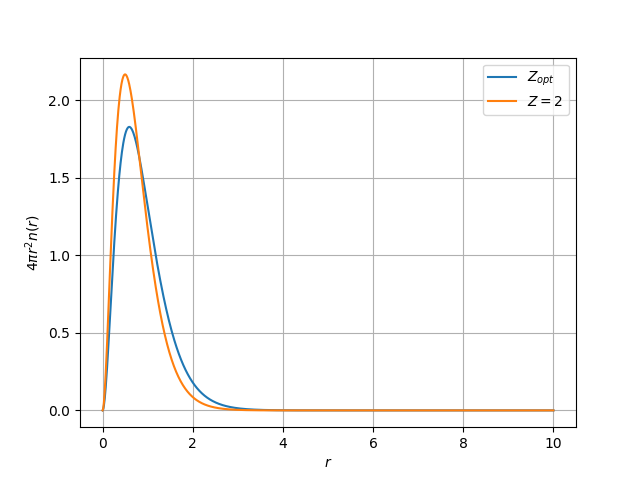
\includegraphics[scale=0.8
    ]{CSE_389D/ps_4/density(1).png}
    \caption{$4\pi r^2n(r)$ vs $r$
}
    \label{fig:enter-label}
\end{figure}

\lstinputlisting[language=python]{"untitled33.py"}

\end{document}